\begin{figure}[ht]
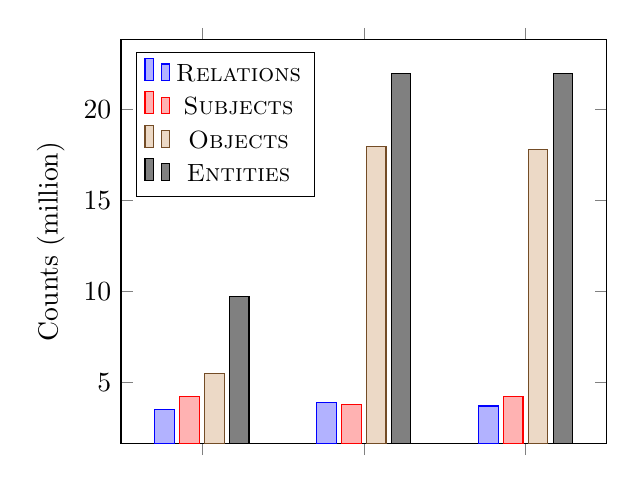
\begin{tikzpicture}
\begin{axis}[
    scale=0.9,
    ybar, 
    enlarge x limits={true, abs value=0.50},
    bar width=7pt,
    legend style={font=\small},
    xtick=data,
    legend pos= north west,
    ylabel=Counts (million),
    xticklabels={
      \reverb, \openie, \openiecoref
    },
]
\addplot 
    coordinates {(1,3.5) (2,3.9) (3,3.7)};
            \addlegendentry{\textsc{Relations}}

\addplot 
    coordinates {(1,4.2) (2,3.8) (3,4.2)};
            \addlegendentry{\textsc{Subjects}}

\addplot 
    coordinates {(1,5.5) (2,18) (3,17.8)};
            \addlegendentry{\textsc{Objects}}

\addplot 
    coordinates {(1,9.7) (2,22) (3,22)};
            \addlegendentry{\textsc{Entities}}

\end{axis}
\end{tikzpicture}
  \caption{
    \label{fig:triples}
    Counts of unique relations, subjects, objects, and entities,
    respectively, where uniqueness is determined by a case
    insensitive string match. The number of unique entities is given by
    the cardinality of the set intersection between subjects and
    objects.
  }
\end{figure}
